\documentclass[oneside,a4paper,14pt]{extarticle}
\usepackage[T1,T2A]{fontenc}
\usepackage[a4paper,letterpaper,top=20mm,bottom=20mm,left=30mm,right=10mm]{geometry}
\usepackage{amsmath, amssymb}
\usepackage[utf8]{inputenc}
\usepackage[russian]{babel}
\usepackage{textcomp}
\usepackage{indentfirst}
\usepackage{graphicx}
\usepackage{float}
\usepackage{mwe}
\usepackage{wrapfig}
\usepackage{caption}
\usepackage{tocloft}
\renewcommand{\cftsecleader}{\cftdotfill{\cftdotsep}}
\usepackage{longtable}
\usepackage{amsmath}
\usepackage{amsfonts}
\usepackage{amsthm}
\usepackage{float}
\usepackage[all]{xy}
\usepackage[breaklinks]{hyperref}
\usepackage{titlesec}
\usepackage{fancyvrb}
\usepackage{paracol}
\usepackage{listings}
\usepackage{xcolor}
\usepackage{listings}

\definecolor{codegreen}{rgb}{0,0.6,0}
\definecolor{codegray}{rgb}{0.5,0.5,0.5}
\definecolor{codepurple}{rgb}{0.58,0,0.82}
\definecolor{backcolour}{rgb}{0.95,0.95,0.92}
\break
\lstdefinestyle{csharpstyle}{
    backgroundcolor=\color{backcolour},
    commentstyle=\color{codegreen},
    keywordstyle=\color{magenta},
    numberstyle=\tiny\color{codegray},
    stringstyle=\color{codepurple},
    basicstyle=\ttfamily\footnotesize,
    breakatwhitespace=false,
    breaklines=true,
    captionpos=b,
    keepspaces=true,
    numbers=left,
    numbersep=5pt,
    showspaces=false,
    showstringspaces=false,
    showtabs=false,
    tabsize=2,
    language=[Sharp]C
}

\lstset{style=csharpstyle}

\titleformat{\section}{\normalsize\bfseries}{\thesection}{1em}{}
\titleformat{\subsection}{\normalsize\bfseries}{\thesubsection}{1em}{}
\titleformat{\subsubsection}{\normalsize\bfseries}{\thesubsubsection}{1em}{}
\renewcommand\baselinestretch{1.33}\normalsize
\setlength{\parindent}{1.25cm}

\begin{document}

\newpage\thispagestyle{empty}
\begin{center}
    МИНИСТЕРСТВО НАУКИ И ВЫСШЕГО ОБРАЗОВАНИЯ\\
    РОССИЙСКОЙ ФЕДЕРАЦИИ\\
    ФЕДЕРАЛЬНОЕ ГОСУДАРСТВЕННОЕ БЮДЖЕТНОЕ\\
    ОБРАЗОВАТЕЛЬНОЕ УЧРЕЖДЕНИЕ ВЫСШЕГО ОБРАЗОВАНИЯ\\
    «ВЯТСКИЙ ГОСУДАРСТВЕННЫЙ УНИВЕРСИТЕТ»\\
    Институт математики и информационных систем\\
    Факультет автоматики и вычислительной техники\\
    Кафедра электронных вычислительных машин
\end{center}

\vspace{20mm}
\begin{center}

    Отчёт по лабораторной работе №2\\
    по дисциплине\\
    «Объектно-ориентированное программирование»\\
\end{center}
\vfill

Выполнил студент гр. ИВТб-2301-05-00 \hfill
\makebox[8cm]{\hrulefill /Ковальский И.И./}

Проверил преподаватель\hfill
\makebox[8cm]{\hrulefill /Шмакова Н.А./}

\vfill
\begin{center}
    Киров\\
    2026
\end{center}
-
\newpage
\setcounter{page}{1}
\tableofcontents
\newpage

\section*{Цель работы}
\addcontentsline{toc}{section}{Цель работы}
Разработка приложения с графическим интерфейсом пользователя на языке C\# с использованием принципов объектно-ориентированного программирования и организацией хранения данных в реляционной базе данных PostgreSQL.

\section*{Задание}
\addcontentsline{toc}{section}{Задание}

На основании согласованной в первой лабораторной работе предметной области разработать приложение с графическим интерфейсом пользователя, используя классы и особенности C\#. Сведения об объектах предметной области необходимо хранить в БД.

Основные требования к выполнению:
\begin{enumerate}
    \item Сохранить все требования первой работы: каждый класс в отдельном файле, наличие базового абстрактного класса, применение наследования. Доступ к полям классов должен осуществляться через свойства (геттеры и сеттеры).
    \item Реализовать графический интерфейс пользователя (Windows Forms).
    \item Для хранения данных использовать базу данных. Данные не должны храниться в одной общей таблице. Должны быть реализованы основные CRUD-функции.
    \item Методы классов из первой работы должны быть доступны для вызова из пользовательского интерфейса.
    \item Описать в отчете структуру классов, включая классы формы, а также особенности подключения и работы с БД.
\end{enumerate}

\newpage

\section*{Выполнение лабораторной работы}
\addcontentsline{toc}{section}{Выполнение лабораторной работы}

\subsection*{Описание предметной области и иерархии классов}
\addcontentsline{toc}{subsection}{Описание предметной области и иерархии классов}

Предметная область сохранена — «Организации». Архитектура приложения разделена на три логических слоя:
\begin{itemize}
    \item классы предметной области:
    \begin{itemize}
        \item Organization - базовый класс организаций.
        \item ComOrg - класс коммерческой организации, наследник Organization.
        \item NonComOrg - класс некоммерческой организации, наследник Organization.
    \end{itemize}

    \item класс доступа к данным - DatabaseHelper;
    \item классы интерфейса - Form1, Program.
\end{itemize}

\begin{figure}[H]
  \centering
  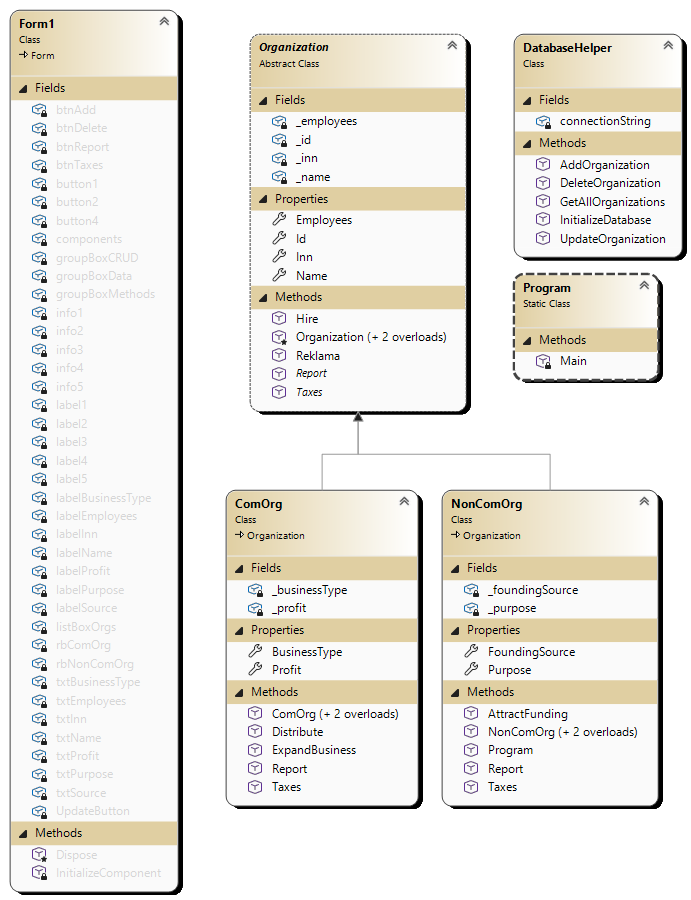
\includegraphics[width=0.8\textwidth]{ClassDiagram1.png}
  \caption{Диаграмма классов}
  \label{fig:class_diagram2}
\end{figure}

\begin{figure}[H]
  \centering
  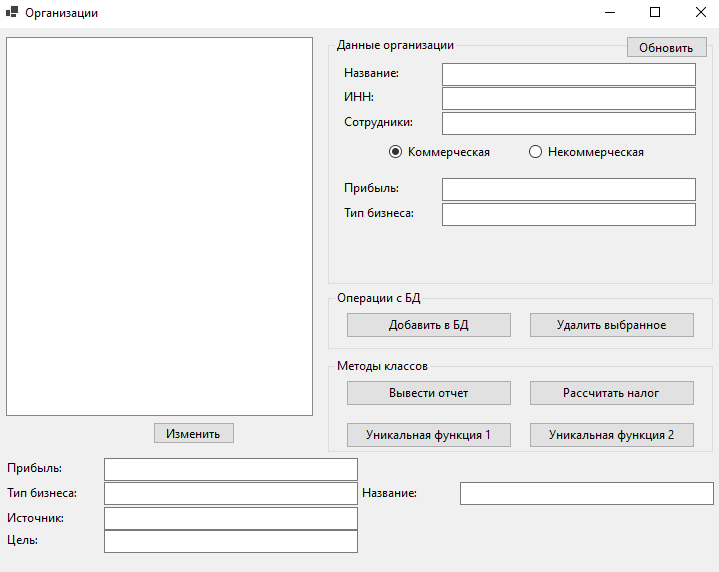
\includegraphics[width=1\textwidth]{Экранная форма.png}
  \caption{Экранная форма программы}
  \label{fig:screen_form}
\end{figure}

\newpage

\subsection*{Описание классов предметной области}
\addcontentsline{toc}{subsection}{Подробное описание классов предметной области}

\subsubsection*{Абстрактный базовый класс Organization: organization.cs}

\textbf{поля:}
\begin{itemize}
    \item private int \_id - уникальный идентификатор организации.
    \item private string \_name - название организации.
    \item private string \_inn - ИНН организации.
    \item private int \_employees - количество сотрудников.
\end{itemize}

\textbf{геттеры сеттеры:}
\begin{itemize}
    \item public int Id - getter public, setter protected. Получение индентифекатора.
    \item public string Name - get и set. Получение и изменение имени.
    \item public string Inn - get и set. Получение и изменение ИНН.
    \item public int Employees - get и set. Получение и изменение числа сотрудников.
\end{itemize}

\textbf{конструкторы:}
\begin{itemize}
    \item protected Organization() - конструктор по умолчанию.
    \\ Устанавливает \_id=0, \_name="Organization", \_inn="1234567890", \_employees=0.
    \item protected Organization(string name, string inn, int employees)\\конструктор с параметрами без идентификатора. \_id=0.
    \item protected Organization(int id, string name, string inn, int employees)
    \\конструктор с идентификатором для загрузки из базы данных.
\end{itemize}

\newpage

\textbf{Абстрактные методы:}
\begin{itemize}
    \item public abstract int Taxes() - Расчёт налога для конкретной организации.
    \item public abstract string Report() - Формирует отчёт об организации.
\end{itemize}

\textbf{Общие методы:}
\begin{itemize}
    \item public void Hire() - Увеличивает \_employees на 1 и выводит сообщение в консоль.
    \item public string Reklama() - Возвращает строку с рекламой вида "\_name оч крутая!".
\end{itemize}

\subsubsection*{Класс ComOrg: comorg.cs}

Наследование: public Organization.

\textbf{поля:}
\begin{itemize}
    \item private string \_profit - прибыль организации.
    \item private string \_businessType - тип бизнеса.
\end{itemize}

Наследуемые поля: \_id, \_name, \_inn, \_employees (доступ через базовый класс).

\textbf{геттеры сеттеры:}
\begin{itemize}
    \item public string Profit - get и set. Получение и изменение прибыли.
    \item public string BusinessType - get и set. Получение и изменение типа бизнеса.
\end{itemize}

\newpage

\textbf{конструкторы:}
\begin{itemize}
    \item public ComOrg() - конструктор по умолчанию.\\
    Вызывает конструктор базового класса с параметрами: name="ООО Дылды", inn="458358238", employees=5. Устанавливает \_profit="100",\\ \_businessType="Розничная торговля".

    \item public ComOrg(string name, string inn, int employees, string profit,\\ string businessType)\\
    Конструктор без идентификатора с собственными и родительскими параметрами.

    \item public ComOrg(int id, string name, string inn, int employees, string profit, string businessType)\\
    Конструктор с идентификатором для загрузки из базы данных.
\end{itemize}

\textbf{Переопределённые методы:}
\begin{itemize}
    \item public override int Taxes() - Пытается преобразовать \_profit в число, затем вычисляет 20\% от прибыли. Если преобразование не удалось, возвращает 0.
    \item public override string Report() - Формирует многострочный отчёт: название, ИНН, количество сотрудников, прибыль, тип бизнеса.
\end{itemize}

\textbf{Собственные методы:}
\begin{itemize}
    \item public string ExpandBusiness() - Увеличивает прибыль на 20\% (прибыль = прибыль + прибыль*20).
    \item public string Distribute() - Вычисляет 3/22 от прибыли (прибыль / 22 * 3).
\end{itemize}

\newpage

\subsubsection*{Класс NonComOrg: noncomorg.cs}

Наследование: public Organization.

\textbf{поля:}
\begin{itemize}
    \item private string \_purpose - цель деятельности организации.
    \item private string \_foundingSource - источник финансирования (гранты, пожертвования и т.п.).
\end{itemize}

\textbf{геттеры сеттеры:}
\begin{itemize}
    \item public string Purpose - get и set.
    \item public string FoundingSource - get и set.
\end{itemize}

\textbf{конструкторы:}
\begin{itemize}
    \item public NonComOrg() - конструктор по умолчанию.\\
    Вызывает конструктор базового класса с параметрами: name="Фонд Помощи", inn="0987654321", employees=10. Устанавливает \_purpose="Помощь нуждающимся", \_foundingSource="Гранты".

    \item public NonComOrg(string name, string inn, int employees, string purpose, string foundingSource)\\
    Конструктор без идентификатора.

    \item public NonComOrg(int id, string name, string inn, int employees, string purpose, string foundingSource)
    \\Конструктор с идентификатором.
\end{itemize}

\textbf{Переопределённые методы:}
\begin{itemize}
    \item public override int Taxes() - Вычисляет налог как employees * 10.
    \item public override string Report() - Формирует многострочный отчёт: название, цель, источник финансирования.
\end{itemize}

\textbf{Собственные методы:}
\begin{itemize}
    \item public string Program(string program) - Просто возвращает переданную строку (имитация проведения программы).
    \item public string AttractFunding(string source) - Возвращает переданный источник (имитация привлечения финансирования).
\end{itemize}

\newpage

\subsection*{Класс доступа к данным DatabaseHelper: BD.cs}
\addcontentsline{toc}{subsection}{Класс доступа к данным DatabaseHelper}

Класс отвечает за подключение к PostgreSQL и выполнение CRUD-операций. Используется библиотека Npgsql.

\textbf{поля:}
\begin{itemize}
    \item private string connectionString - строка подключения к БД (хост, порт, имя БД, логин, пароль).
\end{itemize}

\textbf{методы:}
\begin{itemize}
    \item public void InitializeDatabase() - Инициализирует датабазу.\\
    \textbf{SQL запрос:}
    \begin{lstlisting}
        CREATE TABLE IF NOT EXISTS Organizations (
                            Id SERIAL PRIMARY KEY,
                            Name VARCHAR(255) NOT NULL,
                            Inn VARCHAR(50) NOT NULL,
                            Employees INTEGER NOT NULL,
                            OrgType VARCHAR(50) NOT NULL
                        );

                        CREATE TABLE IF NOT EXISTS ComOrgs (
                            Id INTEGER PRIMARY KEY REFERENCES Organizations(Id) ON DELETE CASCADE,
                            Profit VARCHAR(60),
                            BusinessType VARCHAR(255)
                        );

                        CREATE TABLE IF NOT EXISTS NonComOrgs (
                            Id INTEGER PRIMARY KEY REFERENCES Organizations(Id) ON DELETE CASCADE,
                            Purpose TEXT,
                            FoundingSource VARCHAR(255)
                        );
    \end{lstlisting}
    \item public void AddOrganization(Organization org) - Добавляет организацию в БД. Использует транзакцию: сначала вставка в Organizations с RETURNING Id, затем вставка в соответствующую дочернюю таблицу.\\
    \textbf{SQL запрос:}
    \begin{lstlisting}
        INSERT INTO Organizations (Name, Inn, Employees, OrgType)
                            VALUES (@name, @inn, @employees, @type)
                            RETURNING Id;

    INSERT INTO ComOrgs (Id, Profit, BusinessType) VALUES (@id, @profit, @busType)


    INSERT INTO NonComOrgs (Id, Purpose, FoundingSource) VALUES (@id, @purpose, @source)
    \end{lstlisting}
    \item public System.Collections.Generic.List<Organization> GetAllOrganizations() - Выполняет LEFT JOIN между Organizations, ComOrgs и NonComOrgs, читает результат и по полю OrgType создаёт объекты ComOrg или NonComOrg.\\
    \textbf{SQL запрос:}
    \begin{lstlisting}
        SELECT o.Id, o.Name, o.Inn, o.Employees, o.OrgType,
                               c.Profit, c.BusinessType,
                               n.Purpose, n.FoundingSource
                        FROM Organizations o
                        LEFT JOIN ComOrgs c ON o.Id = c.Id
                        LEFT JOIN NonComOrgs n ON o.Id = n.Id
                        ORDER BY o.Id;
    \end{lstlisting}
    \item public void DeleteOrganization(int id) - Удаляет запись из Organizations, дочерние удаляются каскадно.
    \\
    \textbf{SQL запрос:}
    \begin{lstlisting}
        DELETE FROM Organizations WHERE Id = @id;
    \end{lstlisting}
    \item public void UpdateOrganization(Organization org) - Обновляет данные в базовой и дочерней таблицах внутри транзакции.\\
    \textbf{SQL запрос:}
    \begin{lstlisting}
        UPDATE Organizations SET Name = @name, Inn = @inn, Employees = @emp WHERE Id = @id

        UPDATE ComOrgs SET Profit = @profit, BusinessType = @busType WHERE Id = @id

        UPDATE NonComOrgs SET Purpose = @purpose, FoundingSource = @source WHERE Id = @id
    \end{lstlisting}
\end{itemize}

\newpage

\subsection*{Классы графического интерфейса}
\addcontentsline{toc}{subsection}{Классы графического интерфейса}

\subsubsection*{Класс Form1: Form1.cs, Form1.Designer.cs)}

Главное окно приложения.

\textbf{поля:}
\begin{itemize}
    \item private DatabaseHelper dbHelper - объект для работы с БД.
    \item private System.Collections.Generic.List<Organization> currentOrgs - текущий список организаций, загруженных из БД.
\end{itemize}

\textbf{Компоненты интерфейса (инициализируются в Designer):}
\begin{itemize}
    \item listBoxOrgs - список загруженных организаций.
    \item groupBoxData - группа для ввода данных (поля Name, Inn, Employees, кнопки выбора типа, поля наследников).
    \item groupBoxCRUD - кнопки "Добавить в БД" и "Удалить выбранное".
    \item groupBoxMethods - кнопки "Вывести отчет", "Рассчитать налог", уникальная функция 1, уникальная функция 2.
    \item info1...info5 - Текстовые поля для отображения и редактирования информации выбранной организации.
\end{itemize}

\textbf{Основные методы:}
\begin{itemize}
    \item private void UpdateList() - обновляет listBoxOrgs, загружая данные из БД, используя dbHelper.GetAllOrganizations().
    \item private void ToggleFields() - скрывает или показывает поля ввода в зависимости от выбранного типа организации.
    \item private void UpdateListBoxSelection(object sender, System.EventArgs e) - обработчик выбора элемента в списке. Заполняет текстовые поля info1...info5 данными выбранной организации, настраивает видимость и доступность полей в зависимости от типа.
    \item private void btnAdd\_Click(object sender, System.EventArgs e) - считывает данные из полей ввода, создаёт объект ComOrg или NonComOrg, добавляет в БД, вызывая dbHelper.AddOrganization, обновляет список.
    \item private void btnDelete\_Click(object sender, System.EventArgs e) - удаляет выбранную организацию, используя dbHelper.DeleteOrganization.
    \item private void btnUpdate\_Click(object sender, System.EventArgs e) - обновляет список.
    \item private void btnReport\_Click(object sender, System.EventArgs e) - вызывает метод Report() у выбранной организации и показывает результат в MessageBox.
    \item private void btnTaxes\_Click(object sender, System.EventArgs e) - вызывает Taxes() и показывает результат.
    \item private void btnUnique1\_Click(object sender, System.EventArgs e) - для коммерческой организации вызывает ExpandBusiness() и обновляет прибыль в БД; для некоммерческой вызывает Program().
    \item private void btnUnique2\_Click(object sender, System.EventArgs e) - для коммерческой вызывает Distribute(); для некоммерческой сбрасывает Purpose на "Ничего".
    \item private void button4\_Click(object sender, System.EventArgs e) - сохраняет изменения, внесённые пользователем в поля info1...info5, в выбранную организацию и обновляет БД через dbHelper.UpdateOrganization.
\end{itemize}

\subsubsection*{Класс Program: Program.cs}

Точка входа в приложение, запускает главную форму Form1().

\newpage

\subsection*{Особенности подключения и работы с БД PostgreSQL}
\addcontentsline{toc}{subsection}{Особенности подключения и работы с БД PostgreSQL}

Для хранения данных используется СУБД PostgreSQL. Взаимодействие реализовано с помощью библиотеки Npgsql.

\textbf{Структура таблиц:}
\begin{itemize}
    \item Таблица Organizations хранит общие поля: Id, Name, Inn, Employees, OrgType (тип организации: "ComOrg" или "NonComOrg").
    \item Таблица ComOrgs связана внешним ключом с Organizations по полю Id. Содержит поля Profit и BusinessType.
    \item Таблица NonComOrgs связана аналогично, содержит Purpose и FoundingSource.
    \item ON DELETE CASCADE обеспечивает удаление связанных записей при удалении из Organizations.
\end{itemize}

\textbf{Транзакции:}
При добавлении или обновлении организации используются транзакции, для гарантии сохранности данных в обеих таблицах, либо отмене изменений при ошибке.

\textbf{Загрузка данных:}
При вызове GetAllOrganizations() выполняется LEFT JOIN между тремя таблицами. По полю OrgType создаётся объект соответствующего класса. При этом используется конструктор с идентификатором.\\
\textbf{SQL запрос:}
\begin{lstlisting}
SELECT o.Id, o.Name, o.Inn, o.Employees, o.OrgType,
                               c.Profit, c.BusinessType,
                               n.Purpose, n.FoundingSource
                        FROM Organizations o
                        LEFT JOIN ComOrgs c ON o.Id = c.Id
                        LEFT JOIN NonComOrgs n ON o.Id = n.Id
                        ORDER BY o.Id;
\end{lstlisting}
\newpage

\subsection*{Демонстрация принципов ООП}
\addcontentsline{toc}{subsection}{Демонстрация принципов ООП}

\textbf{Инкапсуляция:}
Все поля классов объявлены как private. Доступ к ним осуществляется через публичные геттеры и сеттеры или методы.

\textbf{Наследование:}
Классы ComOrg и NonComOrg наследуют от абстрактного класса Organization, получая все его поля и методы (Id,  Name, Inn, Employees, Hire(), Reklama()). При этом они переопределяют абстрактные методы Taxes() и Report().

\textbf{Полиморфизм:}
В Form1 все объекты хранятся в списке List<Organization>. При вызове методов Report() или Taxes() через переменную базового типа автоматически выполняется соответствующая реализация из дочернего класса. Также при добавлении в БД метод AddOrganization принимает параметр типа Organization, но внутри определяет реальный тип через оператор is.

\section*{Вывод}
\addcontentsline{toc}{section}{Вывод}

В ходе выполнения второй лабораторной работы консольное приложение на C++ было успешно перенесено на язык C\# с созданием графического интерфейса пользователя. Были выполнены все требования:

Приложение демонстрирует основные принципы ООП и показывает, как можно строить многослойные приложения с графическим интерфейсом и хранением данных в СУБД.

\end{document}